\documentclass[10pt, a4paper]{article}
\usepackage[top=3cm, bottom=3cm, left=2cm, right=2cm]{geometry} % 上下左右距離邊緣 2cm
\usepackage{amsmath, amsthm, amssymb}   % AMS 數學環境
\usepackage{enumitem}   % enumerate itemize
\usepackage{xeCJK}      % 中文
\usepackage{fontspec}   % 設定字體
\usepackage{anyfontsize}    % \fontsize{}{}
\usepackage{graphicx}   % 圖片
\usepackage{caption}    % for \caption*
\usepackage{fancyhdr}   % 頁首頁尾
\usepackage{titlesec}   % 設定 section 字體、\titlespacing
\usepackage{tabularx, makecell} % 加強版表格
\usepackage{hyperref}   % 超連結
\usepackage{xcolor}     % 文字顏色
\usepackage{ulem}       % 底線
\usepackage{eso-pic}    % 圖標
\usepackage{booktabs}   % 表格線條
\usepackage{listings}   % 程式碼上色
\usepackage{indentfirst}    % 縮排
\usepackage{setspace}   % 行間距
\usepackage{seqsplit}   % 換行
\usepackage{fancyvrb}
\usepackage[T1]{fontenc}

% 設定 section, subsection 字體
\titleformat*{\section}{\fontsize{15.5}{15.5}\selectfont\bfseries}
\titleformat*{\subsection}{\fontsize{13}{13}\selectfont\bfseries}

% 設定 math mode 字體
\DeclareMathSizes{10}{12}{7}{5}
\setlength{\mathsurround}{1.0pt}

\XeTeXlinebreaklocale "zh"  % 中文自動換行
\XeTeXlinebreakskip = 0pt plus 1pt  % 文字的彈性間距
\linespread{1.35}\selectfont  % 行距
\setlength{\parskip}{1.8ex} % 段落間距
\setitemize[1]{itemsep=-4pt,partopsep=0pt,parsep=1ex,topsep=5pt} % itemize 間距
\setenumerate[1]{itemsep=0pt,partopsep=0pt,parsep=\parskip,topsep=5pt} % enumerate 間距
\setlength{\parindent}{2em} % 縮排

% 設定 section 左邊的 hspace 以及上下的 vspace
\titlespacing\section{0pt}{12pt plus 4pt minus 2pt}{10pt plus 2pt minus 2pt}
\titlespacing\subsection{0pt}{16pt plus 4pt minus 2pt}{10pt plus 2pt minus 2pt}

% 設定中文字型
\setCJKmainfont[AutoFakeBold=4]{Noto Serif CJK TC} % 一般中文字體
\newcommand{\chfont}{SourceHanSansTW-Bold.ttf} % 標題字體
\setCJKfamilyfont{\chfont}{\chfont}[AutoFakeBold = 3]

% 設定英文字型
% \setmainfont{Times New Roman}
% \usepackage{newtxtext}
\setmonofont{Monaco.ttf}

\newcommand{\myhref}[2]{\textcolor{blue}{\href{#1}{#2}}}
\newcommand{\highlight}[2]{\textcolor{#1}{\textbf{#2}}}
\newcommand{\td}[1]{{\setmainfont{Monaco.ttf}{#1}}}  % 測資、程式碼字體
% \newcommand{\td}[1]{{\begin{spacing}{1.2}\setmainfont{Monaco.ttf}{#1}\end{spacing}}}  % 測資、程式碼字體
\newcommand{\bd}[1]{{\setmainfont{DIN-BoldAlternate Regular.otf}{\CJKfamily{\chfont}#1}}}  % 題目字體

\newenvironment{tests}
    {\VerbatimEnvironment\setlength\parindent{0pt} \setmainfont{Monaco.ttf} \fontsize{11}{11}\selectfont\begin{Verbatim}}% \begin{tests}
    {\end{Verbatim}\par\normalsize}% \end{tests}

\newenvironment{mycenter}[1][\topsep]
    {\setlength{\topsep}{#1}\par\kern\topsep\centering}% \begin{mycenter}[<len>]
    {\par\kern\topsep}% \end{mycenter}

\newcommand{\ContestName}{$111$ 學年度板橋高中資訊學科能力競賽 Round $1$}
\newcommand{\Logo}{
\includegraphics[width=2.4cm]{logo.png}}

\newcommand\AtPageUpperRight[1]{\AtPageUpperLeft{\put(\LenToUnit{0.83\paperwidth},\LenToUnit{-2.7cm}){#1}}}

\newcommand{\newblank}{\newpage\begin{center}\hspace{0pt}\vfill{\fontfamily{cmr}\selectfont\textit{\Large{This page is intentionally left blank.}}}\vfill\hspace{0pt}\end{center}}

%%% 重定義一些 command %%%
\newcommand{\N}{\mathbb{N}}
\newcommand{\Z}{\mathbb{Z}}
\newcommand{\Q}{\mathbb{Q}}
\newcommand{\R}{\mathbb{R}}
\renewcommand{\C}{\mathbb{C}}
\newcommand{\F}{\mathbb{F}}
\renewcommand{\O}{\mathcal{O}}
\newcommand{\floor}[1]{\left\lfloor{#1}\right\rfloor}
\newcommand{\ceil}[1]{\left\lceil{#1}\right\rceil}
\newcommand{\link}[2]{\href{#1}{\textcolor{cyan}{\underline{#2}}}}

\pagestyle{fancy}
\lhead{\ContestName}
\renewcommand{\headrulewidth}{0pt}
\AddToShipoutPictureBG{\AtPageUpperRight{\put(20, -5)\Logo}}
\renewcommand{\arraystretch}{0.8}

\definecolor{codegreen}{rgb}{0,0.6,0}
\definecolor{codegray}{rgb}{0.5,0.5,0.5}
\definecolor{codebrown}{rgb}{0.56, 0.08, 0.0}
\definecolor{backcolour}{rgb}{0.95,0.95,0.92}

\lstdefinestyle{code}{
%    backgroundcolor = \color{backcolour},
    commentstyle = \color{codegreen},
    keywordstyle = \color{codebrown},
    numberstyle = \tiny\color{codegray},
    stringstyle = \color{codepurple},
    basicstyle = \ttfamily\footnotesize,
    breakatwhitespace = false,
    breaklines = true,
    captionpos = b,
%    frame = single,
    keepspaces = true,
    showspaces = false,
    showstringspaces = false,
    showtabs = false,
    tabsize = 4
}

\lstset{style = code}


\begin{document}
\section*{\bd{第四題:數獨(Sudoku) \color{blue}{[此題為 Output Only]}}}
\subsection*{\bd{問題敘述}}
「數獨」是一款益智遊戲,在遊戲的一開始會有一個 $n^2\times n^2$ 的表格,其中這整張表格變切成了 $n^2$ 塊區域,每一塊區域內都有 $n\times n$ 個格子。每個格子可以是空的,也可以包含一個 $1\sim n^2$ 的數字。一個合法的數獨同時會滿足以下條件:
\begin{enumerate}
    \item 所有在同一列的數字皆兩兩相異。
    \item 所有在同一行的數字皆兩兩相異。
    \item 所有在同一子區域的數字皆兩兩相異。
\end{enumerate}
下圖是兩個合法的數獨範例,兩個數獨內皆不包含空的格子:

\begin{figure}[htp]
    \centering
    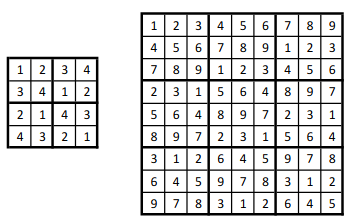
\includegraphics[width=0.5\linewidth]{board.png}
\end{figure}

現在,給你一些尚有一些空格子的合法數獨,請你試圖填入盡可能多的數字並保持該數獨一直都是合法的。保證給定的數獨至少存在一種填滿所有空格子的填數字方法。

本題為一 output only 的任務,並且會部分給分。你將會拿到 10 個輸入檔,說明每一個未完成數獨的樣子。對於每一個輸入檔,你應該繳交一個輸出檔,該檔案描述一組填入一些數字後的成果。對於一個合法的數獨成果,你的成績將依照填入數字的多寡做相應的評分。
\subsection*{\bd{輸入格式}}
每一個輸入檔之格式如下:

首行輸入一個整數 $n$。

接下來 $n^2$ 行,第 $i$ 行將有 $n^2$ 個正整數 $A[i][1]\;A[i][2]\;\cdots\;A[i][n^2]$ 以空格隔開。其中 $0$ 代表該格子為空。
\subsection*{\bd{輸出格式}}
輸出 $n^2$ 行,第 $i$ 行將有 $n^2$ 個正整數 $B[i][1]\;B[i][2]\;\cdots\;B[i][n^2]$ 以空格隔開。代表你填入數字後的成果。
\subsection*{\bd{測資限制}}
\begin{itemize}
    \item $2\le n\le 20$。
    \item $0\le A[i][j]\le n^2$。
    \item 給定的數獨 $A$ 是合法的,且保證至少存在一種填滿所有空格子的填數字方法。
\end{itemize}
\subsection*{\bd{輸入範例 1}}
{
\setlength\parindent{0pt}
\td{
2\\
0 2 0 0\\
3 0 0 0\\
0 0 4 0\\
0 0 0 1
}
}
\subsection*{\bd{輸出範例 1}}
{
\setlength\parindent{0pt}
\td{
4 2 3 0\\
3 1 2 4\\
1 3 4 2\\
2 4 0 1
}
}
\subsection*{\bd{評分說明}}
一個被視為 \bd{「合法」} 的輸出檔,必須滿足以下所有條件:

\begin{itemize}
    \item 所有在同一列的數字皆兩兩相異。
    \item 所有在同一行的數字皆兩兩相異。
    \item 所有在同一子區域的數字皆兩兩相異。
    \item 原本不是 $0$ 的數字依舊保持原樣。
    \item $0\le B[i][j]\le n^2$
\end{itemize}

注意,假設你填出了一個不完整的數獨成果,你並不需要保證存在一種方法可以使剩下的空格子能夠被合法地填滿。

對於每一個合法的輸出檔,你最高可以得到 10 分。令 $A$ 中空格子的數量為 $p$,令 $B$ 中空格子的數量為 $q$,那麼你將根據以下規則得分:

\begin{itemize}
    \item 得 $10\times (p-q)/p$ 分。
\end{itemize}

詳見下表。本題共有 10 個測試資料檔案,條件限制如下所示。
\begin{center}
    \begin{tabular}[t]{@{}cccl@{}}
    \toprule
    測試資料 & 分數 & $n$ & 額外輸入說明\\
    \midrule
    1 & 10 & 2 & 輸入範例 1。\\
    2 & 10 & 3 & 無其他限制。\\
    3 & 10 & 3 & 無其他限制。\\
    4 & 10 & 10 & 無其他限制。\\
    5 & 10 & 20 & $A[i][j]=0$。\\
    6 & 10 & 4 & 無其他限制。\\
    7 & 10 & 8 & 無其他限制。\\
    8 & 10 & 12 & 無其他限制。\\
    9 & 10 & 16 & 無其他限制。\\
    10 & 10 & 20 & 無其他限制。\\
    \bottomrule
    \end{tabular}
\end{center}

\end{document}
